% Copyright 2007 by Till Tantau
%
% This file may be distributed and/or modified
%
% 1. under the LaTeX Project Public License and/or
% 2. under the GNU Public License.
%
% See the file doc/licenses/LICENSE for more details.

\documentclass[portuguese,10pt,xcolor=table]{bredelebeamer}
\setbeameroption{show notes}

\usepackage[brazil]{babel}
\usepackage[utf8]{inputenc}
\usepackage{times}
\usepackage{varwidth}
\usepackage{listings} % Código de programas
\usepackage{tikz}
\usepackage{tikzsymbols}
\usepackage{pifont}
\usepackage[tikz]{bclogo}
\usetikzlibrary{arrows,shapes}

\usetikzlibrary{calc,decorations.pathmorphing,patterns}
\pgfdeclaredecoration{penciline}{initial}{
	\state{initial}[width=+\pgfdecoratedinputsegmentremainingdistance,
	auto corner on length=1mm,]{
		\pgfpathcurveto%
		{% From
			\pgfqpoint{\pgfdecoratedinputsegmentremainingdistance}
			{\pgfdecorationsegmentamplitude}
		}
		{%  Control 1
			\pgfmathrand
			\pgfpointadd{\pgfqpoint{\pgfdecoratedinputsegmentremainingdistance}{0pt}}
			{\pgfqpoint{-\pgfdecorationsegmentaspect
				\pgfdecoratedinputsegmentremainingdistance}%
				{\pgfmathresult\pgfdecorationsegmentamplitude}
			}
		}
		{%TO 
			\pgfpointadd{\pgfpointdecoratedinputsegmentlast}{\pgfpoint{1pt}{1pt}}
		}
	}
	\state{final}{}
}



\everymath{\displaystyle}
\tikzstyle{every picture}+=[remember picture,decoration=penciline]
\DeclareTextFontCommand{\textdf}{\bfseries\color{blue!80}}
%\tikzstyle{every node}+=[decorate]
%\tikzstyle{every path}+=[decorate]
%\tikzstyle{na} = [baseline=-.5ex]

\usepackage[T1]{fontenc}

\def\lecturename{DIM0118 - Introdução às técnicas de programação}

\title{\insertlecture}

\author{Prof. Fernando Figueira\\(adaptado do material do Prof. Rafael Beserra Gomes)}

\institute
{
	UFRN
}

\subject{Funções parte 1}

\lecture[]{Funções parte 1}{}

\date{}

\def\exe[#1]{\color{gray}#1\color{black}}
\def\exp[#1]{\color{gray}<\textit{#1}>\color{black}}
\def\espaco{\color{gray}\hspace{0.2cm}\color{black}}
\def\espaco{\color{blue}␣\color{black}}
\def\inativo[#1]{\color{gray}#1\color{black}}

\definecolor{deepgreen}{rgb}{0,0.5,0}
\lstset{
	language=C,
	basicstyle=\footnotesize\ttfamily,
	%basicstyle=\scriptsize\ttfamily,
	keywordstyle=\footnotesize\bfseries\sffamily,
	%keywordstyle=\scriptsize\bfseries\sffamily,
	showstringspaces=false,
	numbers=left,
	numberstyle=\footnotesize,
	stepnumber=1,
	numbersep=5pt,
	tabsize=4,
	%backgroundcolor=\color{blue!05},
	backgroundcolor=\color{gray!35},
	showspaces=false,
	showtabs=false,
	stringstyle=\ttfamily\color{red!80!brown},
	commentstyle=\ttfamily\color{blue!80},
	keywordstyle=\bfseries\color{deepgreen},
	escapeinside={\%*}{*)}
	}
	\renewcommand{\lstlistingname}{Código}
	\begin{document}

	\usebackgroundtemplate{%
		
\includegraphics[width=\paperwidth,height=\paperheight]{background2}
	}
	\begin{frame}
		\maketitle
		\begin{center}
			\tiny
			Material compilado em \today.\\
			Licença desta apresentação:\\
			
\includegraphics[height=1.0cm]{by-sa.png}\\
			http://creativecommons.org/licenses/
		\end{center}
	\end{frame}
	\def\GN[#1]{\colorbox{gray!40}{#1}}
	\def\RN[#1]{\colorbox{red!40}{#1}}
	\def\BN[#1]{\colorbox{blue!40}{#1}}
	\def\ON[#1]{\colorbox{orange!40}{#1}}
	\def\WN[#1]{\colorbox{white!40}{#1}}

	\section{Funções}

	\begin{frame}
		Escrever na tela o resultado de $2 \times 2^3$\\
			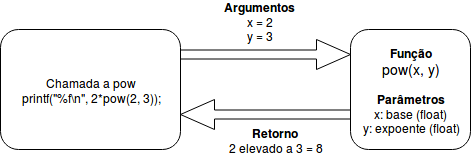
\includegraphics[height=3.0cm]{funcao1.png}\\
	\end{frame} 
	\begin{frame}
		Escrever na tela o resultado de $4^{3^2}$\\
			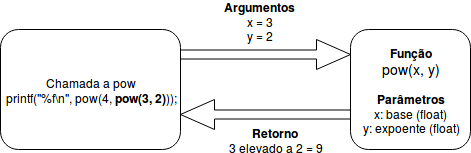
\includegraphics[height=3.0cm]{funcao2.png}\\
	\end{frame} 
	\begin{frame}
		Escrever na tela o resultado de $4^{3^2}$\\
			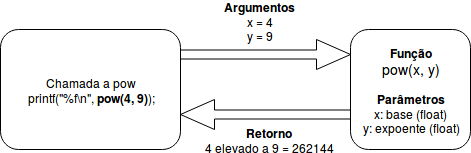
\includegraphics[height=3.0cm]{funcao3.png}\\
	\end{frame} 

	\begin{frame}
		Já utilizamos (\textit{chamamos}) várias funções:
		\begin{itemize}
			\item pow(x, y): \textdf{retorna} $x^y$
			\item sqrt(x): \textdf{retorna} a raiz quadrada de x
			\item printf(...): escreve na saída padrão e \textdf{retorna} a quantidade de caracteres escritos
			\item scanf(...): lê da entrada padrão e \textdf{retorna} a quantidade de elementos lidos com sucesso
			\item malloc(x): reserva x bytes na memória e \textdf{retorna} o endereço base
			\item srand(x): altera a semente para a geração de números aleatórios
		\end{itemize}		
	\end{frame} 

	\begin{frame}
		Quais funções há em C e como utilizá-las?
				\begin{itemize}
					\item as funções estão organizadas em \textdf{bibliotecas}
					\item verifique a \textdf{assinatura} da função\\
						exemplo:        \textdf{double sqrt(double x);}

					\item consulte \textbf{man 3 nomefuncao} ou http://www.cplusplus.com/reference/clibrary/
				\end{itemize}
			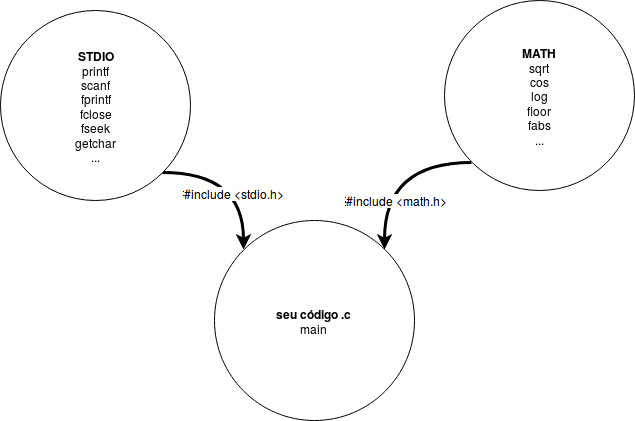
\includegraphics[height=4.5cm]{includes.png}
	\end{frame} 
	\begin{frame}
		Você pode incluir outras bibliotecas, exemplo:
				\begin{itemize}
					\item gtk+: para criar interfaces gráficas
					\item opengl: para gráficos 3D
					\item ...dentre tantas outras
				\end{itemize}
				Provavelmente exigirá a instalação da biblioteca (exemplo, para usar o gtk+ pode fazer no ubuntu: \textit{sudo apt-get install libgtk-3-dev})
			
			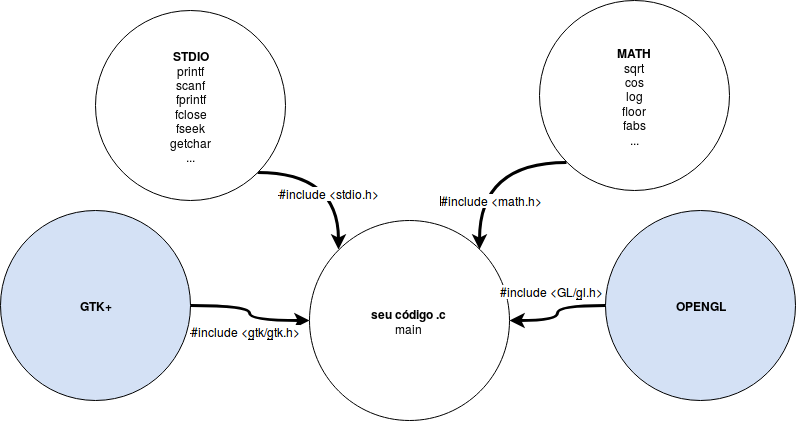
\includegraphics[height=4.5cm]{includes2.png}
	\end{frame}




	%%%%%%%%%%%%%%%%%%%%%%%%%%%%%%%%%%%%%%%%%%%%%%%%%%%%%%%%

	\section{Sintaxe}
	\begin{frame}
		\begin{center}
			\structure{\large Sintaxe para criar funções}
		\end{center}
	\end{frame} 


	\begin{frame}
		\exp[tipo de retorno] identificadorDaFuncao(\exp[params separados por ,]) \{\\
				\espaco \exp[instrução 1]\\
				\espaco \exp[instrução 2]\\
				\espaco \exp[...]\\
				\espaco \exp[instrução n]\\
				\}
				\begin{itemize}
					\item \textdf{Assinatura da função: } o tipo de retorno + identificador da função + parâmetros
					\item A instrução \textdf{return} especifica o valor de retorno e encerra a função
					\item Escolha \textdf{void} caso nada queira retornar
					\item Funções dentro de funções são proibidas em ISO C!
				\end{itemize}
	\end{frame}


	%%%%%%%%%%%%%%%%%%%%%%%%%%%%%%%%%%%%%%%%%%%%%%%%%%%%%%%%
	\section{Exemplos}
		\begin{frame}
			\begin{center}
				\structure{\large Exemplos}
			\end{center}
		\end{frame} 

		\begin{frame}
			Exemplo 1 (Disponível no repositório):
			\lstinputlisting{exemplo1.c}
			\begin{itemize}
				\item \textdf{Nome da função: } soma
				\item \textdf{Parâmetros: } a e b, ambos \textdf{int}
				\item \textdf{Retorno: } \textdf{int} o valor da soma a + b
			\end{itemize}
		\end{frame}

		\begin{frame}
			\begin{alertblock}{\ding{46} Exercício em sala}
				Crie uma função chamada \textbf{maiorDeDois} que receba como \textdf{parâmetros} dois inteiros (\textbf{a} e \textbf{b}) e que \textdf{retorne} o maior deles\\
				Por exemplo: 
				\begin{itemize}
					\item				\textbf{maiorDeDois(5, 2)} deve retornar 5
					\item \textbf{maiorDeDois(5, 7)} deve retornar 7
				\end{itemize}
			\end{alertblock}
		\end{frame}

		\begin{frame}
			Exemplo 2 (Disponível no repositório):
				\lstinputlisting{exemplo2.c}
		\end{frame}


		\begin{frame}
			\begin{alertblock}{\ding{46} Exercício em sala}
				Crie uma função chamada \textbf{escreverIntervalo} que receba como parâmetros dois inteiros (\textbf{a} e \textbf{b}) e que escreva na tela os números entre \textbf{a} e \textbf{b}. Não há valor de \textdf{retorno} (use \textdf{void}).\\
				Por exemplo: \textbf{escreverIntervalo(2, 5)} deve escrever na tela 2 3 4 5.
			\end{alertblock}
		\end{frame}


		\begin{frame}
			Há boas e más escolhas na hora de implementar uma função
			\\Em que aspectos as duas implementações a seguir não são boas?
				\lstinputlisting{funcao1.c}
				\lstinputlisting{funcao2.c}
		\end{frame}


	\begin{frame}
		Por que usar funções? 
		\begin{itemize}
			\item evita repetir código manualmente
			\item facilita alterações
			\item encapsulamento (não precisamos saber as instruções de uma função para usá-la!)
			\item melhor organização do código
		\end{itemize}
	\end{frame}




		%%%%%%%%%%%%%%%%%%%%%%%%%%%%%%%%%%%%%%%%%%%%%%%%%%%%%%%%

	\section{Escopo}
	\begin{frame}
		\begin{center}
			\structure{\large Escopo}
		\end{center}
	\end{frame} 

	\begin{frame}
		Escopo das variáveis:
		\begin{itemize}
			\item \textdf{variáveis locais}: parâmetros e variáveis declarados dentro de funções: podem ser usadas somente \textdf{dentro da função} \footnote{é possível acessar fora da função, mas não pelo identificador declarado}.
			\item \textdf{variáveis globais}: variáveis declaradas fora das funções: podem ser usadas em qualquer parte após a declaração
		\end{itemize}
			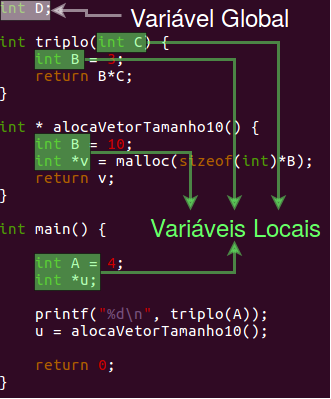
\includegraphics[height=5.0cm]{localVsGlobal.png}\\
	\end{frame}

	\begin{frame}
		Pensando no ciclo de vida dos dados na memória:
				\begin{itemize}
					\item os dados podem estar na região da \textdf{pilha}, do \textdf{segmento de dados}, da \textdf{heap}\\------------------------------
					\item as variáveis globais (declaradas fora das funções) são armazenadas no \textdf{segmento de dados} e valem por todo o programa
					\item as variáveis declaradas dentro das funções e paramêtros são armazenados na \textdf{pilha} e liberados ao encerrar a função
					\item o espaço de memória alocado na \textdf{heap} (usando malloc por exemplo) não é liberado ao encerrar a função
				\end{itemize}
	\end{frame}

	\begin{frame}
		Exemplo de escopo de uma variável declarada dentro de uma função:\\
			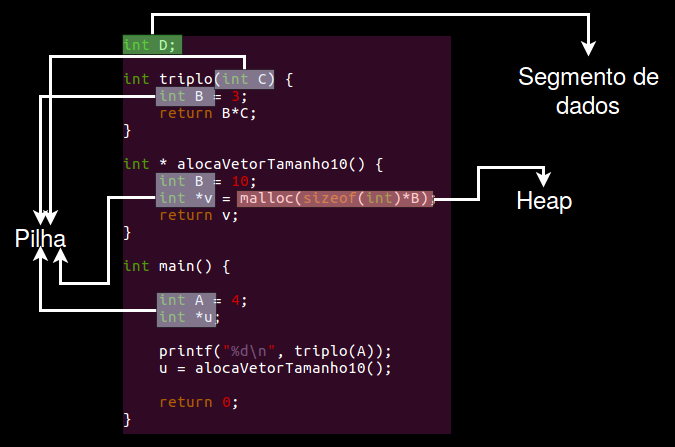
\includegraphics[height=7.0cm]{setoresMemoria.png}\\

	\end{frame}

	%%%%%%%%%%%%%%%%%%%%%%%%%%%%%%%%%%%%%%%%%%%%%%%%%%%%%%%%

	\section{Passagem de parâmetros}
	\begin{frame}
		\begin{center}
			\structure{\large Passagem de parâmetros}
		\end{center}
	\end{frame} 

	\begin{frame}
		Quando uma função é chamada, os argumentos são \textbf{copiados} para os parâmetros (não se referem ao mesmo dado na memória!)\\
				\lstinputlisting{passagem1.c}Disponível no repositório
	\end{frame}

	\begin{frame}
		Passando vetor como parâmetro (opção 1)\\
				\lstinputlisting{passagem2.c}Disponível no repositório
	\end{frame}

	\begin{frame}
		Passando vetor como parâmetro (opção 2)\\
				\lstinputlisting{passagem3.c}Disponível no repositório
	\end{frame}


	\section{A função main}
	\begin{frame}
		\begin{center}
			\structure{\large A função main}
		\end{center}
	\end{frame} 

	\begin{frame}
		\begin{itemize}
			\item A função main é por padrão a executada quando o programa é carregado
			\item Retorna se houve falha no programa (útil para scripts). Então se o programa terminou com sucesso, retorne 0 (falso).
			\item Pode receber \textbf{argumentos de linha de comando}\\
				Exemplo:\\
				\colorbox{gray!30}{./a.out 3 teste 194}\\
				\begin{itemize}
					\item útil para obter dados do usuário já na chamada do programa
					\item alguns comandos do bash utilizam argumentos de linha de comando
				\end{itemize}
		\end{itemize}
	\end{frame}


	\begin{frame}
		Teste o seguinte código (Disponível no repositório):
				\lstinputlisting{args1.c}
				argc é a quantidade de parâmetros de linha de comando e argv um vetor de strings com tais parâmetros
	\end{frame}

	% \begin{frame}
	% 	Teste o seguinte código (Disponível no repositório):
	% 			\lstinputlisting{args2.c}
	% \end{frame}

	
\end{document}

